\section{Adaptive Model Predictive Control for Trajectory Planning} \label{sec:chaser_ampc}
% Following the determination and consensus of the goal states of all chasers, they individually plan trajectories from their start positions to the goal positions. Due to the uncertainty of orbital dynamics due to factors such as the potentially elliptical nature of the orbit, electromagnetic fluctuations, and solar radiation, we propose the application of model predictive control to plan the trajectory of the chaser for rendezvous (initial approach) with the target.
The problem of rendezvous deals with the approach of the chaser from a farther location to a location close to the target.
Due to the uncertainty of orbital dynamics as a result of factors such as the potentially elliptical nature of the orbit, electromagnetic fluctuations, and solar radiation, we propose the application of adaptive model predictive control to plan the trajectory of the chaser for rendezvous (initial approach) with the target.
The uncertainty caused by the elliptical nature of the target's orbit can be traced back to the eccentricity of the orbit.
This orbit can be modeled using the Tshauner-Hempel equations \cite{yamanaka2002new,sinclair2015geometric}
We also consider the effect of non-conservative forces such as (quadratic) atmospheric drag \cite{carter2002clohessy} on the target and the chaser which can be represented using the drag constants of the spacecraft.
These quantities can be formulated as unknown parameters in the problem and learned over time based on the error in the estimated state of the chaser, $\hat{\boldsymbol{r}}$, with respect to its actual state, $\boldsymbol{r}$.
For this purpose, the chaser implements adaptive model predictive control (AMPC) wherein it plans trajectories and updates the calculated trajectory at regular intervals while also updating the estimates for the unknown quantities.

\subsection{Trajectory Planning} \label{ssec:rendezvous-traj-planning}
The rendezvous trajectory planning problem involves generating trajectories such that the goal state is on a sphere around the target; i.e., at a fixed predetermined distance from the target.
% (The sphere can be replaced by any scaled convex shape that completely contains the target as explained later in Section \ref{sec:obs_sphere}.)
The chaser may require one or more intermediate goal locations to observe the target and estimate its physical and inertial properties.
This process of goal radius calculation is repeated for closer rendezvous until the distance between the target and the chaser is sufficiently small enough to initiate docking.
As a result, the trajectory planning problem for rendezvous can be formulated as the following optimization problem:
\begin{subequations}\label{first:main}
\begin{alignat}{2}
    \min_{\boldsymbol{r}, \boldsymbol{u}}\ &J(\boldsymbol{r}(\theta),\boldsymbol{u}(\theta))&&=h(\boldsymbol{r}(\theta_f))\notag\\
    & &&+\int_{\theta_0}^{\theta_f} \left((\boldsymbol{r}(\theta)-\boldsymbol{r}_f)^TQ(\boldsymbol{r}(\theta)-\boldsymbol{r}_f)\right.\notag\\
    & &&\qquad\quad\left.+\boldsymbol{u}(\theta)^TR\boldsymbol{u}(\theta)\right)d\theta\tag{\ref{first:main}}\\
    \textrm{s.t. } & \boldsymbol{r}'(\theta)=A(\theta)\boldsymbol{r}(&&\theta)+B(\theta)\boldsymbol{u}(\theta)+\boldsymbol{d}(\theta),\ \ \boldsymbol{u}\in{\mathbb{U}}\\
    & \boldsymbol{r}(\theta_0)=\boldsymbol{r}_0,&&\\
    &\boldsymbol{r}(\theta)\in{\mathcal{C}}_R\ &&\forall\ \theta\in[\theta_0,\theta_f]\label{eqn:radial-limit-constraint}
\end{alignat}
\end{subequations}
where the system dynamics are given by the extended Tshauner-Hempel equations (explained in Appendix \ref{app:ellp-undrag}), $\boldsymbol{r}_0$ represents the starting point of the chaser, final state cost function $h(\boldsymbol{r}(\theta_f))$ is minimized to move closer to the target, and ${\mathbb{U}}$ represents the range of permissible control input of the chaser.
The additional non-convex 'radial-limit' constraint in Equation \ref{eqn:radial-limit-constraint} ensures that the chaser remains outside all possible locations of the target, hence avoiding collisions.
This is further explained in Section \ref{sec:rendezvous-collision-constraints}.\\
The problem of docking is identical in structure and dynamics to rendezvous.
However, in order to make physical contact feasible, the collision constraints are modified with consideration of the physical (such as the angular velocity) and inertial (such as the moment of inertia) parameters of the target.
As a result, the 'radial-limit' constraint is replaced by a 'target-limit' constraint ${\mathcal{C}}_D$ as explained in Section \ref{sec:time-varying-collision-constraints}.
Moreover, the final state cost function is made stricter to achieve docking with the target.

\subsection{Estimation of Inertial and Angular Parameters of the Target}
\label{sec:target-estimation}
We will observe in Section \ref{sec:time-varying-final-state-constraint} that, at any given time, the final state of the chaser; i.e., the docking position is determined by the current angular position of the target and a predetermined point that is fixed in the body frame of the target.
This point is calculated via optimization of control input as explained in Section \ref{sec:target-deflection}.
(For the sake of this discussion, we consider all angles to be described using Tait-Bryan rotations.)
As a result, it is vital to estimate the inertial and angular parameters of the target.
We do not directly address this problem in this paper.
On the other hand, we encourage the reader to refer to \cite{setterfield2018inertial} on the estimation of such parameters using polhode analysis and similar techniques.\\
However, as observed later in Sections \ref{sec:rendezvous-collision-constraints} and \ref{sec:time-varying-collision-constraints}, although not required for the rendezvous collision constraints, the collision constraint in the docking problem also requires an accurate parameter estimation of the target.
This depends subsequently on the unknown parameters discussed earlier - the eccentricity of the orbit and the drag constant of the target.
In order to estimate these quantities, we introduce adaptive control using set membership identification (SMID).
As explained in \cite{morozov2020performance}, recursive feasibility (meaning that the problem remains feasible for all time) of the MPC operation requires that system uncertainty is monotonically non-increasing throughout adaptation.
This is achieved in our implementation of adaptive control using SMID since the feasible solution set (FSS) shrinks monotonically over time (Refer to Step 2 of Algorithm \ref{alg:smid}).
The progression of estimation using this SMID implementation is demonstrated in Figure \ref{fig:smid}.
\begin{algorithm}
    \textbf{Step 1:} \underline{Generate a Feasible Solution Set (FSS)}\\
    \hspace{2em}\textbf{Step 1a: }$\underline{{\mathsf{e}}}_{est} = \text{\textbf{minimize}}\ {\mathsf{e}}$\\
    \hspace{2em}\textbf{Step 1b: }$      \overline{{\mathsf{e}}}_{est} = \text{\textbf{maximize}}\ {\mathsf{e}}$\\
    \hspace{2em}\textbf{Step 1c: }$\underline{\alpha}_{est}   = \text{\textbf{minimize}}\ \alpha$\\
    \hspace{2em}\textbf{Step 1d: }$      \overline{\alpha}_{est}   = \text{\textbf{maximize}}\ \alpha$\\
    \hspace{4em}such that $\boldsymbol{r}'(\theta)=A(\theta)\boldsymbol{r}+B(\theta)u(\theta)+d(\theta)$\\
    \hspace{5em}$\boldsymbol{r}^P(\theta_0)=\boldsymbol{w}(\theta_0)$, $||\boldsymbol{r}^P(\theta_f)-\boldsymbol{w}(\theta_f)||\leq D$\\
    \hspace{5em}${\mathsf{e}}\in{\mathcal{E}}$, $\alpha  \in{\mathcal{A}}$\\
    \textbf{Step 2:} \underline{Define the new FSS}\\
    \hspace{3em}${\mathcal{E}}_{new}={\mathcal{E}}\cap[\underline{{\mathsf{e}}}_{est}, \overline{{\mathsf{e}}}_{est}]$\\
    \hspace{3em}${\mathcal{A}}_{new}={\mathcal{A}}\cap[\underline{\alpha}_{est},   \overline{\alpha}_{est}]$\\
    \textbf{Step 3:} \underline{Verify the new FSS}\\
    \hspace{3em}attempt to generate $x(t_f)$\\
    \hspace{4em}such that $\boldsymbol{r}'(\theta)=A(\theta)\boldsymbol{r}+B(\theta)u(\theta)+d(\theta)$\\
    \hspace{5em}$\boldsymbol{r}^P(\theta_0)=\boldsymbol{w}(\theta_0)$, $\boldsymbol{r}^P(\theta_f)\approx \boldsymbol{w}(\theta_f)$\\
    \hspace{5em}${\mathsf{e}}\in{\mathcal{E}}_{new}$, $\alpha  \in{\mathcal{A}}_{new}$\\
    \textbf{Step 4:} \underline{Compare and Update the FSS}\\
    \hspace{3em}if Step 3 works:\\
    \hspace{5em}${\mathcal{E}}\leftarrow{\mathcal{E}}_{new}$\\
    \hspace{5em}${\mathcal{A}}\leftarrow{\mathcal{A}}_{new}$\\
    \hspace{3em}else:\\
    \hspace{5em}do nothing\\
    \textbf{Step 5:} \underline{Update Data Range for Adaptation}\\
    \hspace{3em}consider new data by updating $\theta_0$ and $\theta_f$ as:\\
    \hspace{5em}$\Delta\theta = \theta_f - \theta_0$\\
    \hspace{5em}$\theta_0 \leftarrow \theta_f$\\
    \hspace{5em}$\theta_f \leftarrow \theta_f + \Delta \theta$\\~\\
    \caption{Implementation of the \textbf{Set Membership Identification (SMID) algorithm} over several MPC iterations}
    \label{alg:smid}
\end{algorithm}
\begin{figure}[htb]
    \centering
    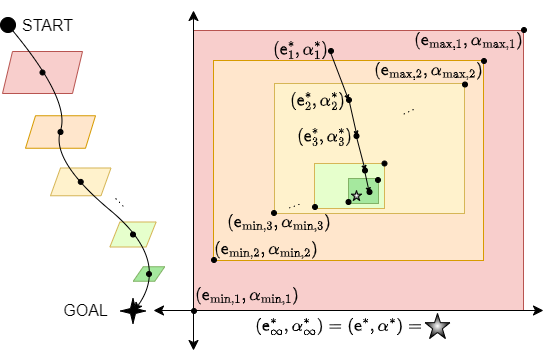
\includegraphics[width=0.98\linewidth]{assets/smid.png}
    \caption{Implementation of the Set Membership Identification (SMID) Algorithm}
    \label{fig:smid}
\end{figure}
We draw motivation from the idea of MSAC-MPC in \cite{tang2023indirect} to stop adaptation after a fixed number of iterations for computational simplicity.
We choose to stop adaptation at the end of rendezvous (before the start of docking) based on the shrunken size of the uncertainty tube.
The time or number of iterations for adaptation can be chosen in practice based on the accuracy of the estimated parameters.\\
We also assume that the intervals considered for the parameters are convex such that every value within two boundary values satisfies convex conditions.
This need not hold true when the intervals are large due to the nonlinear nature of the state space.
As a result, we recommend splitting the intervals such that each sub-interval is convex and treating the new FSS estimate as the union of all feasible sub-intervals.